% !TEX root = ../main.tex


\chapter{Recursion proofs}

This chapter serves as an intermediary background exploration,
diving into more advanced concepts beyond last chapters concepts.
The realm of zero knowledge is dynamic and continuously evolving,
marked by ongoing advancements and active research endeavors. Among these advancements,
recursion proofs is one of the most important and active subjects. Recursion proofs are created to accelerate
the generation of multiple zero-knowledge proofs.
Not all recursion proofs are created equal, they can vary significantly and serve different use cases.
In this section, we will examine these variations, distinguishing between them.
We aim to identify the most suitable method for our daily proof of liabilities and proof of inclusion.


\section{Aggregation}
 %-- Can expend on this using \cite{VRS23}, talk about proof composition
Aggregation is the first and simplest type of recursion for zk proofs. It comprises 2 different phases.
Initially, you create a standard individual proof for multiple blocks. In the second phase, a proof of proof is created.
You could either merge all proofs into a single one, or do a tree-like structure where each parent node proves its child nodes.

This is a quite simple process. Each block as its own proof, and then you prove that the other proofs are valid, giving you only one prove
to verify at the end. Since there are 2 different phases, 2 different circuits need to be constructed.
On the surface, you can parallelize the initial proofs, which decrease the proving time, and you only have one proof to verify, which decreases the verifying time.
However, there are still some issues with aggregation. The most important issue is that the proof time of the second circuit grows linearly with the number of blocks to verify, making it less scalable. \cite{Nova23}
\iffalse
\begin{figure}[H]
   \centering
   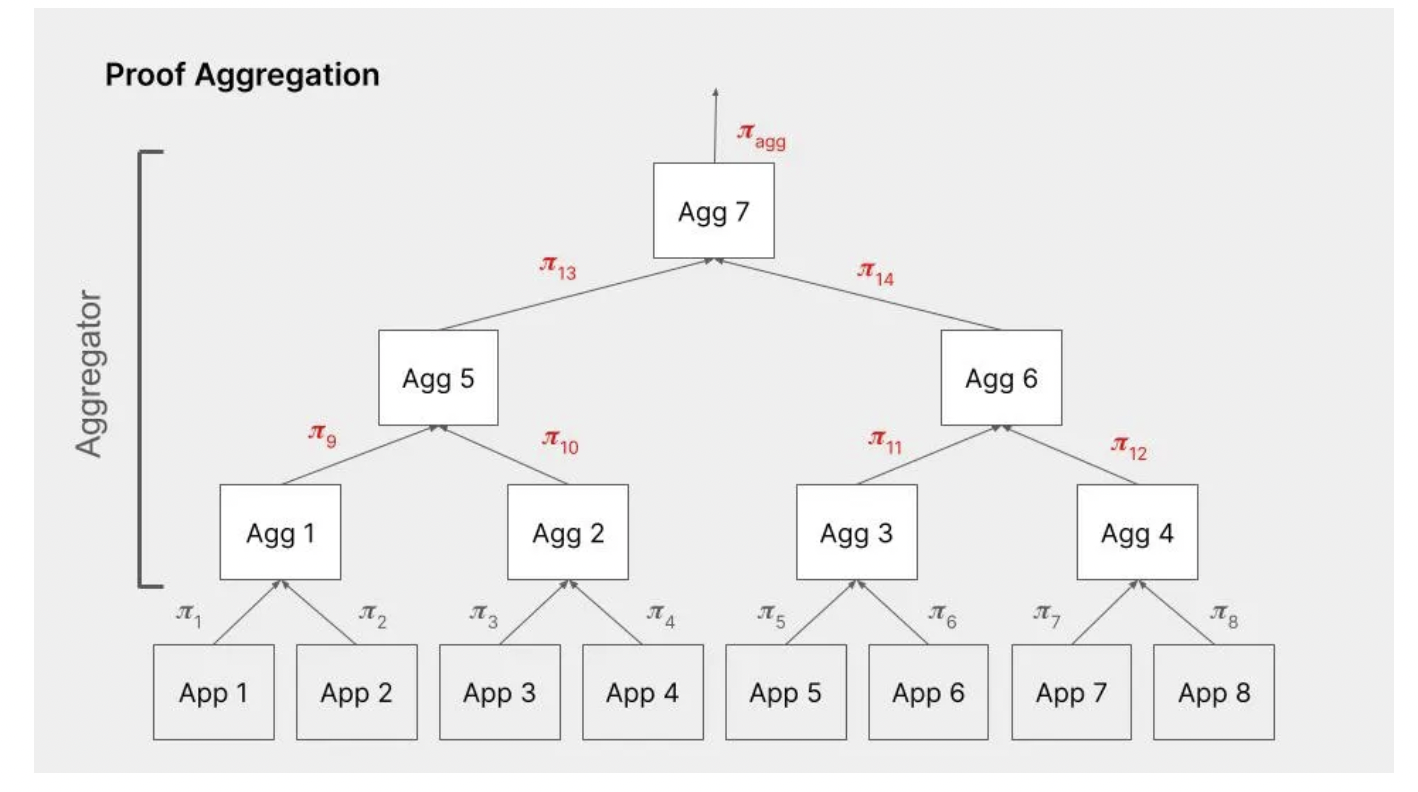
\includegraphics[width=130mm]{AggregationProof.png}
   \caption{Aggregation Proof \cite{TP24}}
   \label{overflow}
   \end{figure}
\fi

\section{Recursion scheme}
The next technique is the recursion scheme, or Incrementally Verifiable Computation (IVC). Like the aggregation, the proof is separated into blocks.
However, in this case each block serves two purposes. Provings that the block itself is valid, and that the previous proof is valid.
The number of constraints will always stay the same because it is only proving 2 things of fixed sizes. This creates
a chain structure, where verifying the latest block is the equivalent of verifying every block in the chain.
It is an improvement from the previous technique, because this allows to maintain a constant number of constraints in the circuit.
This implies that the latest does not take longer to verify than the second block.
However, each block still has to verify the previous block, which takes additional. \cite{Nova23}
%-- Can Expend on this using \cite{VRS23}, talk about IVC


\section{Accumulation}
To mitigate the exponential growth of recursion proofs, the new scheme created by nova differs every computationally heavy task to the end.
All the different parts are accumulated at a later point. Unlike the aggregation scheme, the last part of accumulation does not grow with every new step.
Instead of doing n times heavy work, we are doing it only once.
The heavy part of the verification step in most SNARKS is found when opening the polynomial commitment.


\subsection{Polynomial Commitments}
A polynomial commitment is a cryptographic technique that allows to commit (lock) data, and reveal (unlock) it later.

The commitments are binding, meaning there is no way to alter data once it is committed. They are also significantly shorter than
the data committed. Collisions are inevitable given the vastness of potential data sets mapped onto compact commitments (pigeonhole principle).
However, it is computationally infeasible to find a second dataset matching the same commitment.

The commitments can also be hidden. This means that no information is shared to the receiving party.
An example of a commitment scheme would be to hash a dataset with a collision-resistant hash function such as SHA256, and the hash value is shared.
To add the hiding property, a random string could be added at the beginning of the dataset.

Instead of commiting to a dataset, we could be committing to a polynomial. While a commitment to the coefficient would work, we would be revealing the polynomial
when opening the commitment. We would like to be able to open the commitment only to a certain point of the polynomial.
We are also interested in keeping the polynomial secret. An interesting property of polynomials is that it is evaluable at specific points.
A polynomial commitment is proving to another party that we have a commitment to a polynomial that evaluates to a certain value at a certain point.

Polynomials support linear operations like addition or multiplication. A commitment can be additively homomorphic if the sum of the commitment values
is equal to the sum of the polynomials.

Polynomial commitments are essentials to SNARKs. Verifying opening claims of polynomial commitments constitutes the computationally intensive task we mentioned earlier. \cite{VR23}

\subsection{Halo accumulation}

The concept of deferring the polynomial commitment opening checks, and consolidating them into a single operation, was introduced by Bowe, Grigg, and Hopwood Halo.\cite{BGH23}
The task of checking an opening claim for a polynomial commitment is defined in two steps.
The first part is fast, where you just output a pair of a polynomial and its commitment. The second part is expensive, where we verify the pair $(f_1, c_1)$ of the polynomial $f_1$ and its commitment $c_1$.
The second part can be accumulated if the commitment scheme is additively homomorphic.
Instead of verifying each pair ($c_1$ is a commitment for $f_1$, $c_2$ is a commitment for $f_2$, etc.), we can verify the linear combination of every pairs ($c_1+c_2+...$ is a commitment for $f_1+f_2+...$). \cite{VR23}

\section{Folding scheme}
Nova takes accumulation a step further. Instead of accumulating the hard part at the end, the folding scheme accumulates everything up until the end.
The setup is similar to the recursion scheme, but instead of computing the proof of the previous block, the R1CS are folded together at every block.
Instead of having $n$ set of R1CS, we are left with a single set. The new R1CS are called relaxed R1CS, and are used to compute a single proof at the end of the folding.
\cite{Nova23}  \cite{ASI23}

\subsection{R1CS}
%-- define the different part of a proof (including R1CS)
%-- explain why folding the R1CS is enough for folding the proof
Going back to the previous section, we saw the definition of an arithmetic circuit.
R1CS is simply a representation of an arithmetic circuit.
A R1CS constraint has the form $a*b=y$, where $a$,$b$ and $y$ are combinations of variables.
Lets define our previous \hyperref[subsec:ac]{circuit} as a R1CS:   

\begin{quote}
$w_1 = x_1+x_2+1
\\
w_2 = x_2 -1
\\
x = x_1*w_1*w_2$
\end{quote}

Now the 3rd constraint does not follow the rules, because there are 3 variables being multiplied.
We need to change it using an intermediary value:

\begin{quote}
$w_1 = x_1+x_2+1
\\
w_2 = x_2 -1
\\
w_3 = w_1*w_2
\\
x = x_1*w_3$
\end{quote}
\cite{ZKM3}
If we define $z=(x,w)$, we can express the arithmetic circuit as $ Az \circ Bz = Dz$
where $\circ$ can be define as: $(x_1, x_2) \circ y_1, y_2 = (x_1y_1, x_2y_2)$
\cite{ZKM10}

\subsection{Relaxed R1CS}
The goal is to combine 2 R1CS and obtain another R1CS. If we are able to do that, we can fold every R1CS together and be left with only one.
\\
\\
If we \textbf{define our R1CS}:
\begin{quote}
\textbf{fix an R1CS} program $A,B,D \in \mathbb{F}^{u \times v}_p $
\\
instance 1: public $ x_1 \in \mathbb{F}^n_p $, witness $ z_1 = (x_1, u_1) \in \mathbb{F}^v_p$
\\
instance 2: public $x_2 \in \mathbb{F}^n_p $, witness $ z_2 = (x_2, u_2) \in \mathbb{F}^v_p$
\\
We know $Az_i \circ Bz_i = Dz_i$ for $ i = 1,2$
\end{quote}


\textbf{First attempt}:
\\
Lets define r as a random variable:
\begin{quote}
$r \leftarrow \mathbb{F}_p, x \leftarrow x_1+rx_2$
\\
$z \leftarrow z_1 + rz_2 = (x_1+rx_2, w_1 + rw_2)$
\end{quote}


Then:
\begin{quote}
   $Az \circ Bz = A(z_1 + r z_2) \circ B(z_1 + rz_2)$
   \\
   $= (Az_1) \circ (Bz1) + r^2 (Az_2) \circ (Bz2) + (r(Az_2) \circ (Bz_1) + r(Az_1) \circ (Bz_2))$
   \\
   $=Dz_1 + r^2Dz_2 + E$
   \\
   Where $E$ is a combination of the remaining values.
   \\
\end{quote}
This is not quite an R1CS, because it is not of the form $Az_i \circ Bz_i = Dz_i$.
We need to modify the R1CS so that it can be folded.
\\
\\
Let's \textbf{define a relaxed R1CS}:
\begin{quote}
$A, B,D \in \mathbb{F}^{u \times v}_p, (x \i  \mathbb{F}^n_p, c \in \mathbb{F}_p, E \in \mathbb{F}^u_p) $
\\
Witness: $ z = (x,w) \in \mathbb{F}^v_p s.t. (Az) \circ (Bz) = c(Dz) + E$
\end{quote}
Lets \textbf{fix the R1CS} program once again:
\begin{quote}
$A,B,D \in \mathbb{F}^{u \times v}_p $
\\
instance 1: public $ (x_1,c_1,E_1), $witness$ z_1 = (x_1, w_1) \in \mathbb{F}^v_p$
\\
instance 2: public $(x_2,c_2,E_2), $witness$  z_2 = (x_2, w_2) \in \mathbb{F}^v_p$
\\
We know $(Az_i) \circ (Bz_i) = c_i(Dz_i) + E_i$ for $ i = 1,2$
\end{quote}


\textbf{Second attempt}:
\begin{quote}
$T \leftarrow (Az_2) \circ (Bz_1) + (Az_1) \circ (Bz_2) - c_1(Dz_2) - c_2(Dz_1)$
\\
$x \leftarrow x_1 + rx_2, c \leftarrow c_1 + rc_2, E \leftarrow E_1 + rT +r^2E_2$
\\
$z \leftarrow z_1 + rz_2 = (x_1 +rx_2, w_1 + rw_2)$
\\
$Az \circ Bz = $
\\
$=A(z_1) \circ rB(z_1) +r^2(Az_2) \circ (Bz_2) + r(Az_2) \circ (Bz_1) + r(Az_1) \circ (Bz_2)$
\\
$=c_1(Dz_1) + E_1 + r^2c_2(Dz_2) + r^2E_2+r((Az_2) \circ (Bz_1) + (Az_1) \circ (Bz_2))$
\\
$=(c_+rc_2)(Dz_1+rDz_2)+E_1+r^2E_2+rT$
\\
$=c(Dz) + E$
\end{quote}
We have a valid relaxed R1CS.\cite{ZKM10} \cite{FG23}

